\chapter{ Update-conscious compilation (UCC) techniques}

The conventional compilation takes the following steps to generate binary code from the source code, as depicted in
Figure~\ref{fover.sink}. First, the compiler converts the source code {\tt S} into an intermediate representation {\tt ir}. Next, the compiler optimizes the {\tt ir} for several iterations, and produces the optimized intermediate representation {\tt IR}. Finally, the code generation stage uses {\tt IR} to generate the binary code {\tt E} by applying data allocation, code placement, register allocation, etc.
\begin{figure}[htp]
\centering
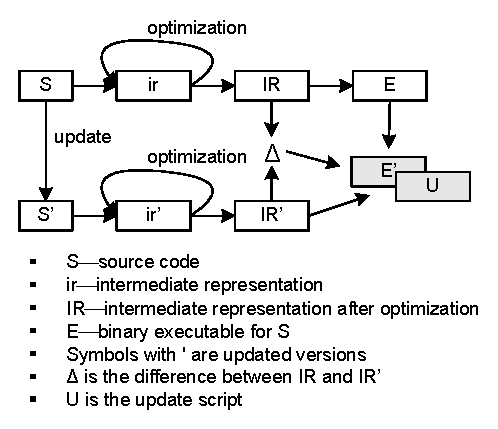
\includegraphics[scale=1]{figures/com_sink.eps}
\caption{The sink-side update-aware compilation.}
\label{fover.sink}
\end{figure}

The proposed UCC schemes are performed at the code generation stage, i.e. from {\tt IR} to {\tt E}. This helps to preserve the performance improvements from the optimization passes. 
Three update-conscious schemes are proposed for register allocation and data allocation phase in the code generation stage. For clarity, I assume that the optimization passes are {\em independent} from these two phases, and other optimizations will be investigated in our future work.

When {\tt S} is updated to {\tt S'} (Figure~\ref{fover.sink}), {\tt ir} and {\tt IR} are also updated to {\tt ir'} and {\tt IR'} respectively. Let $\Delta$ represent the differences between the {\tt IR'} and its previous version {\tt IR}. With $\Delta$, the compiler can analyze and decide how to generate the binary {\tt E'} such that its difference from {\tt E}, denoted as {\tt U}, is small.

The binary difference {\tt U} will then be transmitted over the network to the sensors. When the sensors receive the complete {\tt U}, it will construct the target executable {\tt E'} by combining {\tt U} with old version executable {E}. This demonstrated in Figure~\ref{fover.sensor}.

\begin{figure}[htp]
\centering
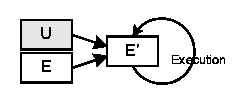
\includegraphics[scale=1]{figures/com_sensor.eps}
\caption{The sensor-side code update and execution.}
\label{fover.sensor}
\end{figure}

\section{Update-conscious compilation for general purpose applications}

In this section, I will discuss about the update-conscious compilation schemes for general purpose applications.
The UCC schemes for general purpose applications include the register allocation scheme, data allocation and
the integrated scheme that covers both register allocation and data allocation.
The goal is to generate the new binary image as similar as the old binary image as possible with the minimal
run-time performance loss. I will discuss about the detailed algorithms in this section.


\subsection{UCC data allocation (UCC-DA) for general purpose applications} 

The executable instructions may need to be updated due to data allocation result changes.
For example, the load/store instructions that access a variable whose memory address is changed
need to be updated.
Thus, one task of UCC is to improve the data allocation similarity.


\subsubsection{Data allocation problem for general purpose applications}

\begin{figure}[htbp]
\centering
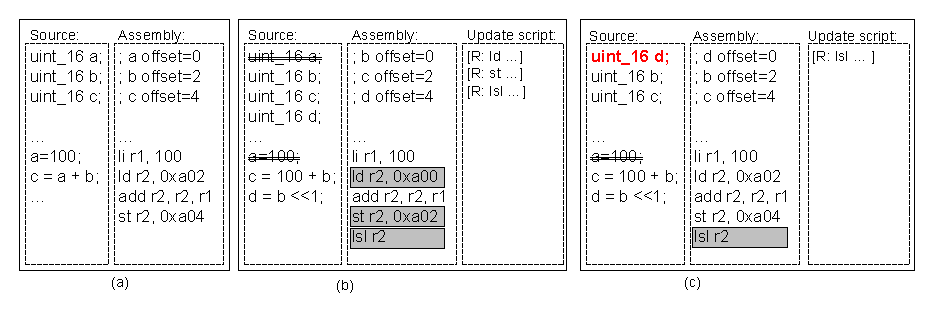
\includegraphics[width=6in]{figures/fdata.0.eps}
\caption{An incremental data allocation example.
(a)original source and assembly code;
(b)new code and the update script;
(c)incrementally generated new code with a smaller update script.}
\label{fdata.0}
\end{figure}

The data allocation
strategy can affect the similarity between different versions of
binary, as illustrated in the example in Figure~\ref{fdata.0}.  In the
original code (Figure~\ref{fdata.0}(a)), three variables {\tt a, b},
and {\tt c} are allocated with offset 0, 2, and 4 respectively, to a
base address. Assume the code is updated by replacing variable {\tt a}
with a constant, and introducing a new variable {\tt d}. The existing
compiler may generate the data allocation scheme as shown in Figure~\ref{fdata.0}(b), in which all variables are assigned with new
offsets, resulting in three update primitives in the update
script. However, an update-conscious algorithm should put the new
variable {\tt d} in {\tt a}'s location, as shown in
Figure~\ref{fdata.0}(c), resulting in only one update primitive in the
script. On the other hand, if there was no {\tt d} in the new code and
if the word taken by {\tt a} was not claimed, I would waste the
word in RAM or more if the function is recursively
invoked on the call stack. This will increase the memory usage on remote sensors.


The memory space here refers to the RAM space, 
which is used to store the call stack. A typical wireless sensor has a
4KB RAM (Mica2 or MicaZ), used to store not only call stack but
also data segment and BSS segment. Figure~\ref{ram} shows the sensor memory
model. The size of the data segment and BSS segment can be calculated
by using static analysis, but the stack size changes as the program
executes. In order to make sure that the stack will not overflow,
the worst case stack size counting the memory waste should satisfy the following equation.

\begin{small}
\begin{equation}
\mbox{\it stack region size}\leq \mbox{\it RAM size} - (\mbox{\it data segment size} + \mbox{\it BSS segment size})
\end{equation}

\end{small}

\begin{figure}[h]
\centering
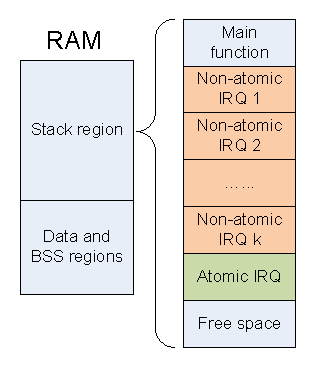
\includegraphics[scale=1]{figures/ram.eps}
\caption{Sensor memory model.}
\label{ram}
\end{figure}

\subsubsection{UCC data allocation for general purpose applications}

To address the problem described above, I propose a {\em
threshold-based data allocation} mechanism~\cite{ucc}.  The intuition is to reuse
the space of deleted variables as much as possible. 
\begin{itemize}
	\item If there are more
new variables than deleted ones, the {\em
threshold-based data allocation} algorithm will first use up the space of the
deleted variables and then allocate more space. 
\item If there are more
deleted variables, some space will be left. 
There are two options to save this space: (i)
relocate some old variables; (ii) do not relocate. The first option
does not waste the space resource on sensor node, but it needs to
change the program code because of the relocated variables. The second
option incurs less code changes but leaves ``holes'' in the call stack 
at runtime. As a hybrid of these two options, the proposed
algorithm keeps the maximal data allocation similarity, under the constraint
that the total wasted RAM space is less than a given threshold --- $SpaceT$. 
This threshold can be calculated by computing the size of each segment 
in RAM using traditional compilation method and subtract that from the RAM 
size.
For ease of illustration, the proposed algorithm
elaborates on the procedures for variables of word type only. The principle can be
applied to other data types such as array and composite structures
similarly.
\end{itemize}

The detailed algorithm is shown in Algorithm~\ref{alg-data}.

\begin{algorithm}
\singlespace
\caption{UCC-Data allocation for general purpose applications.}
\label{alg-data}
\begin{algorithmic}[1]
\singlespace
\REQUIRE Function list $P[*]$, wasted space threshold $SpaceT$.
\ENSURE Data allocation results.
\FORALL{$P_i\in P[]$}
\STATE $Total\_Wasted \leftarrow 0$;
\STATE $DelV_i \leftarrow $ the total number of deleted variables in $P_i$;
\STATE $NewV_i \leftarrow $ the total number of new variables in $P_i$; 
\STATE $InstsNum_i \leftarrow $ the projected maximal simultaneous instances of $P_i$;
\IF {$DelV_i \leq NewV_i$}
\STATE Reuses all the space from deleted variables;
\STATE Allocate extra space to satisfy the remaining new variables;
\ELSE
\STATE Reuses all the space from deleted variables;
\STATE $Extra_i \leftarrow Del_i$ - $NewV_i$;
\STATE $Total\_Wasted$ += $Extra_i \times InstsNum_i$;
\ENDIF
\ENDFOR
\WHILE {$Total\_Wasted > SpaceT$ }
\STATE $Max\_Factor \leftarrow 0$;
\FOR{$P_i \in P[]$ AND $Extra_i > 0$}
\STATE $Usage_i(last) \leftarrow$  the usage of the last variable in $P_i$;
\STATE $Factor_i \leftarrow \frac{InstsNum_i}{Usage_i(last)}$;
\IF {$Factor_i  > Max\_Factor$}
\STATE $Max\_Factor \leftarrow Factor_i$;
\STATE $To\_Move \leftarrow i$;
\ENDIF
\ENDFOR
\STATE Move the last variable in $To\_Move$ to fill up a memory ``hole'';
\STATE $Total\_Wasted$ -= $1\times InstsNum_i$;
\ENDWHILE
\end{algorithmic}
\end{algorithm}

First, it collects the following profiles for each function $P_i(i\geq
0)$ in the program. 
\vspace{+0.1in}
\begin{small}
\begin{center}
\begin{tabular}{r|l}
$DelV_i$ & the total number of deleted variables in $P_i$; \\
$NewV_i$ & the total number of new variables in $P_i$; \\
$InstsNum_i$ & the projected maximal simultaneous instances of $P_i$; \\
$Usage_i(a)$ & the usage of variable {\tt a} in $P_i$. 
\vspace{+0.1in}
\end{tabular}
\end{center}
\end{small}

Second, it gradually allocates new variables within each procedure
$P_i$ as shown in Algorithm~\ref{alg-data} line 6~13. 
Instead of removing the deleted variables directly, it only marks them as deleted variables so that their space can be reused by new variables. If $NewV_i \geq DelV_i$, it reuses all the space from deleted variables and allocate extra space to satisfy
the remaining new variables. If $NewV_i < DelV_i$, i.e., new variables
cannot reuse all space of the deleted ones, then it computes the number of words left to be filled $Extra_i$ = $Del_i$ - $NewV_i$ ,
and moves to the next step.

Third, it adjusts the data allocation by incrementally relocating the
{\em last} variable in each function. It keeps moving the last variable into a
``hole'' left by a deleted variable, until all the ``holes'' are filled.
That is,
\begin{eqnarray}
\sum_{\forall Pi} Extra_i \times InstsNum_i \leq SpaceT
\label{spacet}
\end{eqnarray}

While deciding which function needs to move up the last variable to fill up the ``hole'', 
functions are ordered by two factors.
One is the number of usages of the last variable $Usage_i(last)$ and another one is the number of instances 
that the function can have on stack $InstsNum_i$.

If the last variable in the function is used more often,
such data allocation move will cause more instruction update, so we want
to do the last variable movement to the function whose last variable is
rarely used. Such that, less code update will be triggered.

Another factor is the memory waste. As shown in Figure~\ref{ram}, if a function
has more than one instances on stack. For example, it can be called by both the 
main function and the interrupt handler(s).
One word memory waste in this function may cause 
more than one word RAM waste. Thus, when we have to leave a 
hole in the memory to keep data allocation similarity, we want to
pick up the function that has the smallest number of instances
on the stack, because such decision will cause the least amount
RAM space waste.

\begin{figure*}[h]
\centering
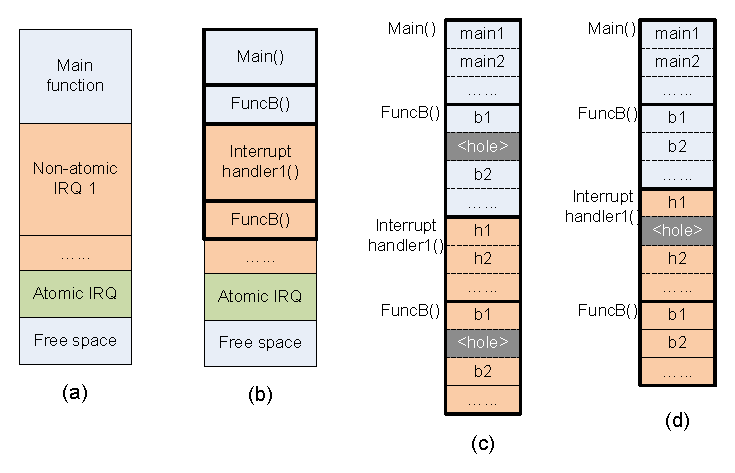
\includegraphics[width=4.5in]{figures/stack.eps}
\caption{RAM usage example.}
\label{stack}
\end{figure*}
Figure~\ref{stack} shows a memory usage example. 
$FuncB()$ is called by both $Main()$ and $Interrupt\_handler1()$, so
it has two instances on the stack, while the other functions only
have one instance. Wasting one word in $FuncB()$ will cause two word
waste in RAM, while wasting one word in $Interrupt\_handler1()$ will
cause only one word waste in RAM. Thus, in order to save RAM usage, we should
move the last variable of function $FuncB()$ instead of $Interrupt_handler1()$.


%As shown in Figure~\ref{fdata.0}, such a move will cause
%changes in all the instructions that use the last variable. If
%equation (~\ref{spacet}) cannot be satisfied for all the procedures, to keep
%the changes minimum, we should first serve those that might demand the
%most runtime memory but have the least number of uses.  That is, we
%should find a procedure $j$ such that

With such consideration, the function $j$ that we pick should satisfy the following
formula.
\begin{small}
\begin{eqnarray}
{{InstsNum_j}\over{Usage_j(last)}} = MAX( {{InstsNum_i}\over{Usage_i(last)}} )~~~ {(\forall i, Extra_i>0)}
\label{factor}
\end{eqnarray}
\end{small}

After we decide which function we will pick, we then relocate the last 
variable in procedure $j$ to one
deleted memory word. By doing so, we can shrink the maximal runtime
memory usage by $InstsNum_j$ (as it is the last variable in that
procedure), and incur less code changes (as the variable with less
usage is selected). We then decrement $Extra_j$ and continue this step
until equation (\ref{spacet}) is satisfied.

For example in Figure \ref{fdata.0}, if {\tt d} is not introduced, we
will reuse {\tt a}'s space with {\tt c} if $SpaceT=0$, i.e. no wasted
space. This will result in an edit script with two primitives to
update {\tt c} and {\tt d} respectively. This code still outperforms
the default scheme in Figure \ref{fdata.0}(b) which requires three
update primitives.

%The data allocation problem may become more complicated if it is
%coupled with code generation where data offset are encoded with
%instruction types. For example successive instructions using
%post-increment addressing (PIA) mode will access successive data in
%memory with implicit address increment between two instructions. If
%data is relocated, new instructions must be inserted to change the
%memory access address in the next instruction.  Fortunately, we
%experimented with {\tt gcc 3.4.3} compiler and found that the PIA mode
%is mainly used to access the four bytes of an integer variable and
%thus is insensitive to the variable relocation. For this reason, we do
%not consider the impact the PIA mode when relocating the data. If they
%are used beyond a word boundary, we treat them individually by
%inserting new addressing instructions.


\subsection{Update-conscious register allocation (UCC-RA) for general purpose applications}
Besides the data allocation results, the register allocation results can also 
affect the similarity between generated binary images.
Instructions need to be updated if the assigned registers are changed.
Thus, another task of UCC is to produce similar register assignment
when generating the new binary.

\subsubsection{Register allocation problem for general purpose applications} 
%

Figure~\ref{freg0} illustrates why different register
allocation decisions can greatly impact the code similarity, and therefore the
update cost. In this example, two variables {\tt a} and {\tt b}
initially have disjoint live ranges and can be allocated to the same
register {\tt R1} (Figure~\ref{freg0}(a)). Assume a small code change
extends {\tt b}'s live range into {\tt a}'s. If there are enough free
registers, a modern register allocator will assign different registers
to them, as depicted in Figure~\ref{freg0}(b).  Variable {\tt b} is
assigned to a new register {\tt R2}, resulting in a name change for
all the uses in subsequent statements in the statement range \{5,15\}.
In contrast, an alternative {\em update-conscious} decision may
allocate {\tt b} to {\tt R2} only for the range \{5,11\} where {\tt
R1} is not free, and match the old allocation for the range \{12, 15\}
with one extra {\tt mov} instruction, as shown in Figure~\ref{freg0}(c). By comparing these two solutions, it is clear that
while the solution (b) achieves better code quality, the solution (c)
results in less update cost. The discrepancy in energy consumption
between data transmission and instruction execution makes the solution
(c) more appealing as it consumes less energy unless the code is very
frequently executed, or the update is extremely rare.

\begin{figure}
\centering
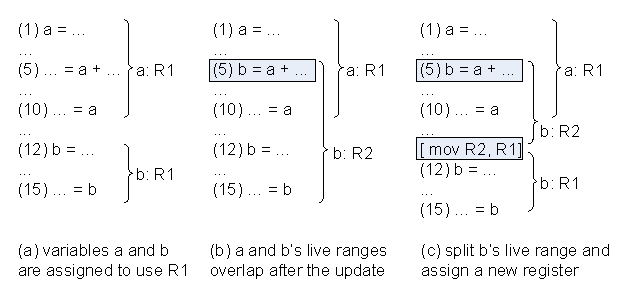
\includegraphics[scale=1.2]{figures/freg.0.eps}
\caption{Allocating different registers for improved energy efficiency.
(a). Variable {\tt a} and {\tt b} are assigned with register {\tt R1};
(b). The live ranges of {\tt a} and {\tt b} overlap with each other after the code update;
(c). Split {\tt b}'s live range and assign a new register to it.}
\label{freg0}
\end{figure}


\subsubsection{UCC register allocation for general purpose applications}\label{secra}
%

The basic idea of UCC register allocation (UCC-RA)~\cite{ucc} is to retain mostly the old register assignments and perform new register allocations to changed and new instructions {\em with preferences to the decisions for the given binary}. 

To achieve this, IR instructions are first identified as ``changed'' or ``non-changed'', and then group successive instructions of the same type into chunks. The register allocator then allocates registers for each chunk.
Decisions for ``changed'' chunks are made by the UCC-RA while decisions for ``unchanged'' chunks are taken from the old code before the update. For the variables whose live ranges span across the chunk boundary, the register allocation consistency is checked at the end. Inter-register movement instructions may be added to ensure the the semantic correctness.

While doing UCC-RA, each variable in the input chunk is tagged with the register name that was assigned in the old binary. This tag is called {\em Preferred-register tag}. The {\em preferred-register tag} is a hint to improving code similarity in UCC-RA.

The register allocator then allocates registers for each changed chunk, and gradually matches the register assignment, or allocation decisions from both changed and non-changed chunks for semantic correctness. Decisions for changed chunks are made by our UCC-RA while decisions for unchanged chunks are taken from the old code before the update. The two decisions are made conjointly. If a variable's live range spans across the chunk boundary, from ``changed'' to ``non-changed'' or vice versa, then the assignment in the ``changed'' chunk gives {\em preference} to the assignment in the ``non-changed'' chunk to maximize the similarity. However, this preference may not always be adopted by the allocator. If the allocator decides to use a new register in the ``changed'' chunk, then a {\tt mov} instruction between the two chunks should be inserted to move data between the new and the old registers. Register preference should also be given to the same variables on different control flow paths (they might be of different chunk types). However, if the allocator chooses a different register, then a {\tt mov} instruction is also necessary.

Clearly, placing too many inter-register movement instructions requires not only transmitting more update data to remote sensors but also executing more instructions at runtime. Therefore it is desirable to develop a precise cost-benefit model such that an inter-register movement instruction is inserted only if it is estimated to be energy-efficient.

\paragraph{Formalizing the UCC register allocation}
Motivated by the 0/1 integer linear programming research for register allocation \cite{related:ilp}, the UCC-RA problem can be formulated as a non-linear integer programming problem. The general idea of how to select the decision variables, formulate the constraints and the objective function is addressed the below. Please refer to my paper \cite{ucc} for details.

{\underline{\em The decision variables.}} 
I use a set of decision variables that represent the register assignments we need to make at each program point. The decision variable is defined as~\ref{decision_vars}. 

\begin{small}
\begin{eqnarray}
X_{op.v.s}^{Ri} = \left\{\begin{array}{r@{\quad:\quad}l}
0  & \mbox{Assertion is true.}\\
1  & \mbox{Assertion is false.}
\label{decision_vars}
\end{array}\right.    
\end{eqnarray}

\begin{center}
\begin{tabular}{c|p{2.0in}} 
$op$ & operation;\\
$v$ &  variable;\\
$s$ & statement; \\
\end{tabular}
\end{center}
\end{small}

The decision variables $X_{op.v.s}^{Ri}$ can be 0 or 1.
With the value assigned to be 1, it means that register {\tt Ri} is assigned to variable {\tt v} at statement {\tt s} for operation {\tt op}, and 0 otherwise. For example, when decision variable $X_{def.v.s}^{Ri}$ is set to 1, it means that the variable {\tt v} is defined at statement {\tt s}, and  register {\tt Ri} is assigned to hold the value of variable {\tt a}. 
In the example shown in Figure~\ref{freg0}(b) statement (1), the decision variable that is used to determine whether
to allocate {\tt R1} for variable {\tt a} can be written as $X_{def.a.1}^{R1}$.

{\underline{\em The objective function.}}
Let us use a simple example in Figure \ref{freg0} to explain our proposed procedure. The code contains several instructions: the first two are the definitions of variable {\tt a} and {\tt b} respectively, while the third one uses both variables. Let us assume at statement (6), {\tt a} is dead but {\tt b} is still alive, and the preferred-registers of {\tt a} and {\tt b} are {\tt R1} and {\tt R2} respectively.


For the code chunk in Figure \ref{freg0}(a), we first introduce a set
of decision variables that represent the register assignments we need
to make at each program point. For example, If variable {\tt a} is allocated to
register {\tt R1} at statement (1), then we have $X_{def.a.1}^{R1}=1$
and $\forall Ri, Ri\neq R1, X_{def.a.1}^{Ri}=0$. Here
$X_{def.a.s}^{Ri}$ is a decision variable to show if variable {\tt a}
is assigned to the register {\tt Ri} at statement {\tt s}. A decision
variable $X_{*}^{*}$ can take value 0 or 1, with 1 meaning that the
corresponding assertion is true, and 0 otherwise. As another example,
if we decided to insert an instruction ``{\tt mov R2 to R3}'' for {\tt
b} before statement (4), we set $ X_{mov.out.b.4}^{R2}=1$,
$X_{mov.in.b.4}^{R3}=1,$ and all other {\tt mov} decision variables
$X_{mov.*.b.4}^{*}$ as 0. As discussed, such a {\tt mov}
instruction may be inserted to release {\tt R2} for other variables,
or to match the old assignment of {\tt b} to {\tt R3} after statement
(4).  The following is a full list of decision variables that we used in
UCC-RA.
\begin{figure}[htbp]
\begin{tabular}{c|p{5.0in}} 
$a / s / Ri$  & variable {\tt a} / statement {\tt s} / Register {\tt Ri} (1$\le$i$\le$31); \\
~\\

$X_{mov.out.a.s}^{Ri}$ & if {\tt a} is moved from {\tt Ri}
to another register at {\tt s}; \\

$X_{mov.in.a.s}^{Ri}$ & if {\tt a} is moved from another
register to {\tt Ri} at {\tt s}; \\

~ \\

$X_{def.a.s}^{Ri}$ & if {\tt a} is allocated to {\tt Ri} at its
definition point {\tt s};\\

$X_{cont.a.s}^{Ri}$ & if {\tt a} is allocated to {\tt Ri} after its
def point {\tt s}; \\

$X_{lastUse.a.s}^{Ri}$ & if {\tt a} is allocated to {\tt Ri} at its
last use point {\tt s} and {\tt a} is dead after {\tt s}. \\

$X_{use.a.s}^{Ri}$ & if {\tt a} is allocated to {\tt Ri} at {\tt s},
but not in {\tt Ri} after {\tt s}; statement {\tt s} is not the last
use.\\

$X_{useCont.a.s}^{Ri}$ & if {\tt a} is allocated to {\tt Ri} at {\tt
s}, and is also in {\tt Ri} after {\tt s}; statement {\tt s} is not
the last use.\\

~ \\

$X_{st.a.s}^{Ri}$ & if {\tt a} is spilled from {\tt Ri} to memory
after {\tt s};\\

$X_{ld.a.s}^{Ri}$ & if {\tt a} is loaded from memory to {\tt Ri}
before its use point {\tt s}; \\

$X_{cont.a.s}^{mem}$ & if the variable is kept in memory after the
statement {\tt s};
\end{tabular}
\caption{Decision variables used in UCC-RA.}
\end{figure}

When defining proper decision variables, we aim to keep their total
number small so that the solver takes less time to find a
solution. For example, we introduce two decision variables
$X_{mov.in.a.s}^{Ri}$ and $X_{mov.out.a.s}^{Ri}$ instead of a more
intuitive $X_{mov.a.s}^{Ri\leftarrow Rj}$ (move {\tt a} from {\tt Rj}
to {\tt Ri} at statement {\tt s}) because of the following reason.
Assume there are 31 registers; the one-variable definition would
introduce $31\times30$ {\em mov} decision variables for each variable
at a program point. This will increase the problem size and slow down
the solver. Instead, we decouple the {\tt mov}'s source register from
the destination register such that only $31\times 2$ decision
variables are required. Then, we simply combine correctly the
corresponding move-in and mov-out variables to implement the register
move.

{\underline{\em The constraints.}}  
With above decision variables, we convert the register allocation
problem into a problem of assigning value 0 and 1 to these
variables. To ensure that the value assignment can be mapped back to a
valid register assignment, these variables are subject to a set of
constraints.

We first define the constraints for variable definitions.  Each
variable should be allocated to one and only one register at its
definition point. Thus we have, for each variable {\tt a} at its
definition point {\tt s}, one and only one $X_{def.a.s}^{Ri}$ can be
1, or,

\begin{small}
\begin{eqnarray}
\sum_{\forall Ri} X_{def.a.s}^{Ri} = 1.
\end{eqnarray}
\end{small}

To ensure valid inter-register movements, we define constraints on
{\tt mov} decision variables as well. Since we may and may not insert
a move instruction at a program point; and the move-in and move-out
decision variables should appear in pairs, we have:

\begin{small}
\begin{eqnarray}
\sum_{\forall Ri} X_{mov.out.a.s}^{Ri} \leq 1  \nonumber \\
\sum_{\forall Ri} X_{mov.out.a.s}^{Ri} = \sum_{\forall Ri} X_{mov.in.a.s}^{Ri}
\end{eqnarray}
\end{small}

At a statement {\tt s}, variable {\tt a} may be loaded from the
memory, or come from inter-register movement. After defining the
variable, the value in the register may be spilled to the memory, or
moved to another register, or stay for later use. Thus we have:

\begin{small}
\begin{eqnarray}
X_{st.a.s}^{Ri} \leq X_{def.a.s}^{Ri} + X_{mov.in.a.s}^{Ri} \nonumber \\
X_{mov.out.a.s}^{Ri} \leq X_{def.a.s}^{Ri}  \nonumber \\
X_{cont.a.s}^{Ri} \leq X_{def.a.s}^{Ri} + X_{mov.in.a.s}^{Ri} 
\end{eqnarray}
\end{small}

For the code spill at a definition point, only a store instruction may
be possibly generated. Thus, we have:

\begin{small}
\begin{eqnarray}
X_{cont.a.s}^{mem} \leq \sum_{\forall Ri}X_{st.a.s}^{Ri}
\end{eqnarray}
\end{small}

We next define the constraints for variable uses. Since we can know if
a use is the last use (through backward analysis),
$X_{lastUse.a.s}^{Ri}$ is always exclusive from
$(X_{use.a.s}^{Ri}+X_{useCont.a.s}^{Ri})$. In addition,
$X_{use.a.s}^{Ri}$ and $X_{useCont.a.s}^{Ri}$ are exclusive, and a use
should be in a register. The above are specified as:

\begin{small}
\begin{eqnarray}
\sum_{\forall Ri} X_{lastUse.a.s}^{Ri} = 1;  ~~~~or \nonumber \\
\sum_{\forall Ri} (X_{use.a.s}^{Ri} + X_{useCont.a.s}^{Ri}) = 1;
\end{eqnarray}
\end{small}

At a use point, a variable may be located in a register due to its use in the
previous instruction, or loaded from the memory, or moved
from another register. Depending on whether it is the last use, we
have one of the following two constraints:

\begin{small}
\begin{eqnarray}
X_{use.a.s}^{Ri} + X_{useCont.a.s}^{Ri} \leq X_{cont.a.{\bf(s-1)}}^{Ri} + X_{ld.a.s}^{Ri} + X_{mov.in.a.s}^{Ri} \nonumber 
\end{eqnarray}
\end{small}
\vspace{-0.1in}
\begin{small}
\begin{eqnarray}X_{last.a.s}^{Ri} \leq X_{cont.a.{\bf(s-1)}}^{Ri} + X_{ld.a.s}^{Ri} + X_{mov.in.a.s}^{Ri} 
\end{eqnarray}
\end{small}

Since we only generate load spill, or inter-register movement
before the use point, we have:

\begin{small}
\begin{eqnarray}
\sum_{\forall Ri}X_{ld.a.s}^{Ri} \leq X_{cont.a.{\bf(s-1)}}^{mem} \nonumber \\
\sum_{\forall Ri}X_{mov.out.a.s}^{Ri} \leq X_{cont.a.{\bf(s-1)}}^{Ri}
\end{eqnarray}
\end{small}

The following constraints are used to ensure that one register is assigned to
only one variable at a time.

$U_{a.s}$ is defined to describe the register assignment to the variable {\tt a}
at instruction {\tt s}.

\begin{small}
\begin{eqnarray}
U_{a.s} = \left\{\begin{array}{r@{\quad:\quad}l} 
X_{def.a.s}^{Ri} & \mbox{if {\tt a} is defined at {\tt s}} \\ 
X_{use.a.s}^{Ri} + X_{useCont.a.s}^{Ri} & \mbox{if {\tt a} is used at {\tt s}} \\
X_{lastUse.a.s}^{Ri} & \mbox{if {\tt a} is used at {\tt s} and no longer used in the later instructions}\end{array}\right. 
\end{eqnarray}
\end{small}

$V_{a.last\_s}$ is defined to show the register assignment information of the last access
point of variable {\tt a}. 
Depending on whether instruction {\tt last\_s} is a defintion point or use point of variable {\tt a}, 
$V_{a.last\_s}$ is calculated in two different ways.

\begin{small}
\begin{eqnarray}
V_{a.last\_s} = \left\{\begin{array}{r@{\quad:\quad}l} 
X_{cont.a.last\_s}^{Ri} & \mbox{if {\tt a} is defined at {\tt last\_s}} \\ 
X_{useCont.a.last\_s}^{Ri} &\mbox{if {\tt a} is used at {\tt last\_s}} \end{array}\right. 
\end{eqnarray}
\end{small}

To make sure that there is no register assignment conflict between the current
variable and the active variables which are processed before, the following constraint
is applied:

\begin{small}
\begin{eqnarray}
\sum_{\forall var}V_{var.last\_s} + U_{a.s} \leq 1 
\end{eqnarray}
\end{small}

For example, the following equations show the constraints at statement (2) in
Figure \ref{freg0}:
\begin{small}
\begin{eqnarray}
U_{b.2} = X_{def.b.2}^{Ri}\nonumber\\
V_{a.last\_use} = X_{cont.a.1}^{Ri}\nonumber \\
thus, ~~X_{def.b.2}^{Ri} + X_{cont.a.1}^{Ri} \leq 1
\end{eqnarray}
\end{small}

Also in order to avoid the register assignment conflict between the variables which
are used in the same instruction, the following constraint needs to be applied:
\begin{small}
\begin{eqnarray}
\sum_{\forall var}U_{var.s} \leq 1 
\end{eqnarray}
\end{small}

For example, the following constraints at statement (6) in Figure \ref{freg0}:

\begin{small}
\begin{eqnarray}
U_{a.6} = X_{lastUse.a.6}^{Ri}\nonumber\\
U_{b.6} = X_{use.b.6}^{Ri} + X_{useCont.b.6}^{Ri} \nonumber\\
thus, ~~X_{lastUse.a.6}^{Ri} + X_{use.b.6}^{Ri} + X_{useCont.b.6}^{Ri} \leq 1
\end{eqnarray}
\end{small}

For Mica2 micro controllers, we need to enforce another type of
constraint. Each register in Mica2 has 8 bits, i.e. one byte. A
32-bit integer variable should be allocated to four {\em
consecutive} registers, i.e., byte {\tt a}, {\tt a}+1, {\tt a}+2, and
{\tt a}+3 should be in register {\tt Ri}, {\tt Ri}+1, {\tt Ri}+2, and {\tt
Ri}+3 respectively:

\begin{small}
\begin{eqnarray}
X_{use.(a).s}^{Ri} = X_{use.(a+1).s}^{R_{i+1}} \nonumber \\
X_{use.(a+1).s}^{Ri} = X_{use.(a+2).s}^{R_{i+1}} \nonumber \\
X_{use.(a+2).s}^{Ri} = X_{use.(a+3).s}^{R_{i+1}} 
\end{eqnarray} 
\end{small}

At the boundary of changed and unchanged code chunks, and at the merge
point of control flows, we insert inter-register move instructions to
make sure that the values are in proper registers before their next
uses. In our future work, instead of performing inter-register
movements, we will introduce constraints similar to those in
\cite{related:ilp} for the merge point of control flows.




{\underline{\em The objective function.}}
\begin{figure}[htbp]
\begin{normalsize}
\begin{center}
\begin{tabular}{r|p{5in}} 
$E_{trans}$ & the energy consumed to disseminate one instruction in WSN; \\
$E_{exe}$ & the energy consumed to execute one instruction.
We use the averaged number here and differentiate the memory access 
(load,store) and ALU instructions in the implementation. \\
~ & \\
$prefer(a, s)$ & the preferred-register for variable {\tt a} at statement {\tt s}; \\
$freq(s)$ & the execution frequency count of statement {\tt s}; \\
~ & \\
$chg(s)$ & if {\tt s} is an unchanged IR instruction.
chg(s)=1 if {\tt s} has been changed; =0 otherwise;\\
$spill(a, Ri, s)$ & if variable {\tt a} was spilled to {\tt Ri}/loaded back from {\tt Ri} 
at statement s in the old binary; 
\end{tabular}
\caption{Notations used in the objective function.}
\label{notation.obj}
\end{center}
\end{normalsize}
\end{figure}
The goal of our integer programming is to minimize the objective
function on total energy consumption, as expressed in equation (\ref{totalE}) in
Figure~\ref{feqn}. The equation defines the total energy consumption of the
changed IR chunk under different register allocation decisions. The notations
used in equation ({\ref{totalE}}) are listed in the right column.
Other terms are explained as follows.

\begin{figure*}[htbp]
\begin{small}
\begin{eqnarray}
E_{total} = 
chg(s) \times E_{changed\_IR} + (1-chg(s))\times E_{unchanged\_IR} +
E_{spill} + E_{extra}  \label{totalE}
\end{eqnarray}
where
\begin{eqnarray}
E_{changed\_IR} &= &\sum_{\forall s} (freq(s) \times E_{exe}) +
\sum_{\forall s}(E_{trans})  \label{cE}\\
%
E_{unchanged\_IR} &= & \sum_{\forall s} (freq(s) \times E_{exe}) + \nonumber\\ 
									&  & \sum_{\forall s}(1-\prod_{\forall a}{X_{def/use.a.s}^{prefer(a,s)}}) \times 					E_{trans} \label{uE}\\
%
E_{spill} &=& \sum_{\forall s, a, Ri}
(freq(s) \times (X_{st.a.s}^{Ri}+X_{ld.a.s}^{Ri}) \times E_{exe}) + \nonumber\\
					& & \sum_{\forall s, a, Ri}( (1-spill(a,Ri,s)) \times
 (X_{ld.a.s}^{Ri}+X_{st.a.s}^{Ri}) \times E_{trans})  \\
E_{extra} &=& \sum_{\forall s, a, Ri}
(freq(s) \times X_{mov.in.a.s}^{Ri} \times E_{exe}) + \nonumber\\
					& &\sum_{\forall a, s, Ri} (X_{mov.in.a.s}^{Ri} \times E_{trans}) 
\end{eqnarray}
\end{small}
\caption{The objective function.}
\label{feqn}
\end{figure*}

$E_{spill}$ specifies the energy consumption due to code spill. It
includes two components: the execution energy and the dissemination
energy. The former has to do with the code quality which is the main
goal of many existing allocators. The latter is not negligible when a
new spill is generated or an old spill is removed. It is zero for all
other cases, i.e. either (1-$spill(a,Ri,s)$)=0 or
$(X_{ld.a.s}^{Ri}+X_{st.a.s}^{Ri})=0$ in the equation (13).  For
example, if {\tt a} is spilled to {\tt R1} in both new and old
binaries, then we have zero transmission cost:

\vspace{+0.1in}
\begin{tabular}{l}
for R1, 1-spill(a,R1,s)=0, $X_{ld.a.s}^{R1}+X_{st.a.s}^{R1}$=1\\ for
Ri(Ri$\neq$R1), 1-spill(a,Ri,s)=1,$X_{ld.a.s}^{Ri}+X_{st.a.s}^{Ri}$=0
\\
\end{tabular}
\vspace{+0.1in}

$E_{changed\_IR}$ specifies the energy consumption due to changed IR
instructions. It includes both the execution and the dissemination
energy consumption as well. As we can see, no matter which register
allocator is used, a changed IR instruction always results in a binary
instruction that should be disseminated to remote sensors. Therefore
$E_{changed\_IR}$ is a constant in the model.

$E_{unchanged\_IR}$ specifies the energy consumption due to unchanged
IR instructions. Assume we have an unchanged IR instruction ``{\tt
a=a+b}'' and {\tt a} and {\tt b}'s preferred-registers are {\tt R1}
and {\tt R2} respectively. If the new allocation decision follows the
old allocation scheme, then there is no dissemination cost, i.e. the
same binary instruction ``{\tt add R1, R2}'' is generated. If {\tt a}
is assigned to a different register, say {\tt R3}, and we generate
``{\tt add R3, R2}'', then this new instruction needs to be
disseminated to replace the old one on the sensor. As shown in
equation (12), this component is non-linear ---- one $E_{trans}$ is
introduced for either one or two changes of the two preferred
registers.

$E_{extra}$ is the extra energy consumption due to inserted
inter-register movements. This term is zero if a traditional compiler
decision is used. Our UCC-RA targets at achieving overall energy efficiency,
i.e. $E_{extra}$ is positive only when we can gain more reduction from
other components, e.g. $E_{unchanged\_IR}$.

In the above model, $X_{*}^{*}$ are decision variables that need to be
determined by the UCC-RA, while others such as $chg(s), freq(s),$
etc.  are known for a given code chunk.  Since equation (12) is
non-linear, the above formulation of UCC-RA results in a mixed integer
non-linear programming problem (MINLP) \cite{bonmin}.  While the speed
of MINLP solvers has been improved greatly in recent years
\cite{bonmin}, it is still much slower than solving a linear problem.  Our
experiments results show that MINLP can be orders of magnitude slower
than a linear problem of similar sizes, i.e., similar number of
decision variables and constraint. We next discuss how to convert the
MINLP problem to an ILP problem through approximation.

\paragraph{Solving an ILP problem}
In this section we model the update energy consumption
linearly such that the UCC-RA can be solved using an ILP
solver. 




For an unchanged IR instruction with two variables {\tt a} and {\tt b}
(to comply with Mica2 AVR ISA, each IR instruction in our model has at
most two different operands). Assume their preferred registers are
{\tt R1} and {\tt R2} respectively, I model the energy consumption as

\begin{small}
\begin{equation}
\sum_{\forall s}(1-X_{use.a...}^{R1} + 
1-X_{use.b...}^{R2})  \times E_{trans} \times \delta 
\end{equation}
\end{small}
\noindent
where $\delta=3/4$, a coefficient that approximates the update cost.
It is decided as follows. Assume each variable has equal opportunity
of being assigned and not assigned to its preferred register. For the
instruction with two variables {\tt a} and {\tt b} and preferred
registers {\tt R1} and {\tt R2} respectively, there are four
possibilities altogether: (i) {\tt a} is in {\tt R1}, {\tt b} is in
{\tt R2}; (ii) {\tt a} is in {\tt R1}, {\tt b} is not in {\tt R2};
(iii) {\tt a} is not in {\tt R1}, {\tt b} is in {\tt R2}; (iv) {\tt a}
is not in {\tt R1}, {\tt b} is not in {\tt R2}. It is clear that case
(i) has no update cost while each of other three cases needs to update
one instruction. Therefore the averaged update cost is $
(3/4)~\times~Cost_{single}$, which decides $\delta$ to be $3/4$.

After converting the model into an ILP problem, I adopt a widely used
ILP solver --- LP\_solve \cite{lpsolve} to find the optimal assignment
of decision variables such that the cost (modeled in the objective
cost function) is minimized.  I then map decision variables back to
register assignments, and generate the code and the corresponding
update script as well.

\subsection{Integration of the UCC data allocation and register allocation}\label{integration}

When constructing the objective function of the update-conscious register allocation scheme (UCC-RA),
the changed and unchanged IR statements are treated differently.For the changed IR statements, the code update cannot be avoided, thus, using UCC-RA scheme cannot
gain any benefit for this type of statements. On the other hand, for the unchanged IR statements, 
whether keeping the register assignment the same as the old version or not will determine whether
it is necessary to update the generated binary instruction(s).  Parameter $chg(s)$ is used 
differentiate these two kinds of IR statements.

With the consideration of the update-conscious data allocation scheme (UCC-DA), we can see that
for the unchanged IR statements, not only the register allocation results but also the data allocation 
results may affect the transmission energy consumption. If the unchanged IR statement is a memory access instructions,
and the memory address of the operand is changed, no matter how the register allocation is done, the
update energy cannot be waived, thus, the objective function $E_{total}$ for this statement should be
formated using formula~\ref{cE} instead of formular~\ref{uE} in Figure~\ref{feqn}.

Based on this observation, I propose two solutions to integrate UCC-DA and UCC-RA schemes for general purpose
applications below. One is an accurate ILP based solution and another one is a light weight heuristic based solution.


\subsubsection{ILP based integration}
In order to integrate the UCC-DA and UCC-RA solutions for general purpose applications,
I first introduce a new decision variable to describe whether to reallocate a variable
or not, then the related constraints and the revised objective function.


{\underline{\em Decision variable $X_{a}^{realloc}$.}}
I define a new decision variable that determines whether to allocate the variable in 
a different memory slot from the old version. 
The decision variable is written as $X_{a}^{realloc}$, and {\tt a} presents the
variable name. If the value is set to ``0'', the memory slot used to hold the
value keeps the same; otherwise, it is changed.


{\underline{\em Data allocation related constraints.}}
As described in the UCC-DA algorithm~\ref{alg-data}, there are two constraints
for UCC-DA decision variables, and I formulate those constraints using the notations
shown in Figure~\ref{notation3} as below.
\begin{figure}[htbp]
\begin{tabular}{c|p{5.0in}} 
$X_{a}^{realloc}$ & if {\tt a} is allocated with a different memory slot from the old version; \\
$InstsNum_i$ & the projected maximal simultaneous instances of procedure $Pi$;\\
%$Usage_i(a)$ & the usage of variable {\tt a} in $Pi$;\\
$Extra_i$& the wasted memory space of procedure $Pi$;\\
$DelV_i$ & the total number of deleted variables in $Pi$;\\
$NewV_i$ & the total number of new variables in $Pi$.\\
\end{tabular}
\caption{Notations used in the ILP based integration.}
\label{notation3}
\end{figure}

The total wasted space on the call stack cannot go beyond the threshold $SpaceT$~\ref{spacet}.
This constraint is formulated as Figure~\ref{dataconsts}.
$DelV_i$ and $NewV_i$ are the number of variables that are removed and inserted
in procedure $Pi$, so they are constants for each $Pi$.
$InstNum_i$ represents the projected maximal simultaneous instances of procedure $Pi$,
which is also a constant. 
The new variables are firstly used to fill up the holes created by deleting variables.
If there are fewer new variables than deleted variables, the unchanged variables
in this procedure can be reallocated to fill up the memory ``holes''.
The wasted memory space of procedure $Pi$ is presented in equation~\ref{wastes},
which is equal to the number of deleted variables minus the number of new variables,
then minus the number of reallocated variables.

\begin{figure*}[ht]
\begin{small}
\begin{eqnarray}
Extra_i = \left\{\begin{array}{r@{\quad:\quad}l}
0  & \mbox{$DelV_i \leq NewV_i$}\\
DelV_i - NewV_i -{\sum\limits_{\forall a}{X_{a}^{realloc}}}&  \mbox{$DelV_i > NewV_i$}
\end{array}\right.  \label{wastes} \\
\sum_{\forall Pi}{Extra_i\times InstsNum_i } \leq SpaceT 
\end{eqnarray}
\end{small}
%\caption{Data allocation constraints.}
%\label{dataconsts}
\end{figure*}


Another constraint is that it always allocates the last variable in each procedure first until the
space constraint is met. This constraint is formulated as equation~\ref{last}.
\begin{figure*}[ht]
\begin{small}
\begin{eqnarray}
\forall{a,b} \;\; old\_addr(a) \leq old\_addr(b)\Rightarrow  X_{a}^{realloc} \leq X_{b}^{realloc}\label{last}
\end{eqnarray}
\end{small}
%\caption{Data allocation constraints.}
%\label{dataconsts}
\end{figure*}



{\underline{\em Integrated objective function.}}

The objective function of the UCC-RA problem is formulated as equation~\ref{totalE}.
There are four parts in the objective function.
The energy consumption of the {\tt ALU} instructions is formulated as $E_{changed\_IR}$ and $E_{unchanged\_IR}$.
The energy consumption of the {\tt spill} instructions is formulated as $E_{spill}$.
The energy consumption of the inserted {\tt mov} instructions is formulated as $E_{extra}$.
Because the data allocation result will only affect the transmission energy consumption of the load/store
instructions, only $E_{spill}$ needs to be reformulated.

In the old formular, there were two factors that determine whether the corresponding load/store instruction needs transmission energy
to update the instruction:
whether there was a spill here in the old binary ($spill(a,Ri,s)$), and how the variables are allocated in the registers($X_{ld.a.s}^{Ri}$ and $X_{st.a.s}^{Ri}$).
For the instructions that did not have the register spill in the old binary, the code
update is required, because this load/store instruction is a newly inserted instruction.
Otherwise, the energy consumpiton depends on whether the register allocation results
are the same as the old one.
In short, only when variables $X_{ld.a.s}^{Ri}$ or $X_{st.a.s}^{Ri}$ and $spill(a,Ri,s)$
are set to be ``1'', the transmission energy can be saved.

Now, besides these factors, whether to reallocate the variable in memory will also
affect the transmission energy.
When the variable is reallocated in memory, which means $X_{a}^{realloc}$
is set to ``1'', the corresponsing load/store instruction needs update
no matter how the other factors are set.
In other words, the instruction update is not necessary, 
only when $spill(a,Ri,s)$ is set to be ``1'' which means this instruction was a 
{\tt spill} instruction in the old binary, 
$X_{ld.a.s}^{Ri}$ or $X_{ld.a.s}^{Ri}$ are set to ``1'' which means that the new
register allocation result is the same as the old binary, 
and  $X_{a}^{realloc}$
is set to ``0'' which means the variable is not reallocated in memory.
Otherwise, this instruction needs to be transmitted.
Thus, the energy consumption of the load/store instructions is then reformulated as equation~\ref{newspill}.

\begin{figure*}[ht]
\begin{small}
\begin{eqnarray}
E_{spill} &=& \sum_{\forall s, a, Ri}
freq(s) \times (X_{st.a.s}^{Ri}+X_{ld.a.s}^{Ri}) \times E_{exe} + \nonumber\\
					& & \sum_{\forall s, a, Ri}(1-spill(a,Ri,s)\times
 (X_{ld.a.s}^{Ri}+X_{st.a.s}^{Ri})\times (1-X_{a}^{realloc}))\times E_{trans} \label{newspill} 
\end{eqnarray}
\end{small}
\caption{Objective function used in the heuristic based integration.}
\label{newObj2}
\end{figure*}

As you can see, the energy function $E_{spill}$(~\ref{newspill}) is no longer a linear function
due to the addition of another decision variable $X_{a}^{realloc}$.
In order to reduce the time spent solving the problem, we need to convert
it into a linear function that will give us an approximated result but 
consumes much less time.
Similar as what we did before in subsubsection~\ref{secra}, $E_{spill}$(~\ref{newspill2})
can be rewritten as below:
\begin{figure*}[ht]
\begin{small}
\begin{eqnarray}
E_{spill} &=& \sum_{\forall s, a, Ri}
freq(s) \times (X_{st.a.s}^{Ri}+X_{ld.a.s}^{Ri}) \times E_{exe} + \nonumber\\
					& & \sum_{\forall s, a, Ri}(1-spill(a,Ri,s)\times
 (X_{ld.a.s}^{Ri}+X_{st.a.s}^{Ri}+1-X_{a}^{realloc})\times \delta )\times E_{trans} \label{newspill2} 
\end{eqnarray}
\end{small}
\caption{Converted objective function used in the heuristic based integration.}
\label{newObj2}
\end{figure*}

Here, $\delta$ is an coefficient that approximates the update cost when we 
convert the integer non-linear problem into an integer linear problem.
Same as in subsubsection~\ref{secra}, we set $\delta$ here to be 3/4.


\subsubsection{Heuristic based integration}

The introduction of the memory reallocation decision variable $X_{a}^{realloc}$ will add $N$ 
decision variables to the ILP problem, where $N$ is the number of variables used in the
program. This will increase the complexity of the ILP problem, thus, increase the
compilation time.
Based on this observation, I design another heuristic based integration algorithm, that
does the data allocation and register allocation separately. This scheme will not
affect the complexity of the ILP problem, because no more decision variables will be introduced.
The detailed algorithm is described as below.

Instead of solving both data allocation and register allocation problems together, 
the compiler will solve them one by one in sequential order. It does UCC-DA first and find out the variables whose 
memory addresses are changed. This information is then passed to the UCC-RA. The memory access statements that
access these variables will not be considered as unchanged IRs.

I introduce another notation $datachg(s)$~\ref{notation2} to describe whether the unchanged IR
statement needs update because of data allocation result changes. After the UCC-DA is done, the compiler marks the variables whose memory location are changed. Then, $datachg(s)$ parameter of the memory access statement that accesses any of these variables is marked as ``1''. Otherwise, it is marked as ``0''.
\begin{figure}[htbp]
\begin{normalsize}
\begin{center}
\begin{tabular}{r|p{5in}} 
$datachg(s)$ & if statement $s$ is a memory access statement and the memory address of the operand is changed
from the old version.
\end{tabular}
\caption{ Notation used in the heuristic based integration.}
\label{notation2}
\end{center}
\end{normalsize}
\end{figure}

The objective function needs to be changed as shown in Figure~\ref{newObj}. When both $chg(s)$ and $datachg(s)$ are set to ``0'' , the IR statement is treated as an unchanged statement.
\begin{figure*}[ht]
\begin{small}
\begin{eqnarray}
chgIR(s) =1-(1-chg(s))\times(1-datachg(s))\\ 
E_{total} = 
chgIR(s) \times E_{changed\_IR} + (1-chgIR(s))\times E_{unchanged\_IR} +
E_{spill} + E_{extra} 
\end{eqnarray}
\end{small}
\caption{Objective function used in the heuristic based integration.}
\label{newObj}
\end{figure*}

The heuristic based solution is easy to implement, however, the result may not be optimal.
While doing UCC-DA, the compiler does not have any information of the UCC-RA result.
It assumes that reallocating a variable in memory will always increase 
code update overhead and makes a local optimal solution yet may not be the global
optimal solution.

For example, assume that we have two data reallocation options. Reallocating variable
{\tt a} and {\tt b} gives the equal amount memory space usage, but variable {\tt a}
is more frequently used than {\tt b}. The UCC-DA is more likely to reallocate variable
{\tt b} instead of {\tt a}, because this decision will cause less code update.
However, if later the UCC-RA decides the register used to hold the value of {\tt a}
needs to be changed, then these {\tt a} related instructions still cannot
avoid being updated. It is more energy efficient to reallocate variable {\tt a} instead
of {\tt b} while doing UCC-DA.

For this type of cases, the ILP based solution can produce a near-optimal solution, 
because it solves the UCC-RA and UCC-DA problems at the same time. However, it will
take longer time. This is the tradeoff between the two proposed algorithms.

\section{Update-conscious compilation for DSP applications}

As discussed in Chapter~\ref{chap:related}, with the address generation unit (AGU), DSP instruction set supports the post-incremental, post-decremental, and pre-decremental instructions,  where address calculated can be in parallel with the other operations. If the next memory location to be accessed is within the auto modify range of the previous access,
no extra address calculation instruction is needed.
Thus, an optimal data allocation algorithm is desired to allocate the variables accessed sequentially in adjacent memory slots. So that, less instructions are needed to explicitly update the address registers, which will reduce the code size and execution overhead.

Because of such connection between the data allocation and code generation in DSP applications, keeping data allocation similar as the older version will keep the addressing modes similar as the old version,
as well as the generated binary image. Therefore, an update-conscious data allocation scheme is desired for DSP application updates.

Besides that, how to assign address registers to the variables can also affect the generated binary similarity.
Keeping the register allocation result similar as the old version also improves the generated binary similarity, which reduces the patch size.

\subsection{Data allocation problem for DSP applications}

An motivation of the proposed UCC data allocation (UCC-DA) scheme is shown in  Figure~\ref{csoa}. When a DSP application undergoes a small update, the code before and after the change are similar. Update oblivious schemes generate the new memory layout and its corresponding binary code without considering the similarity between different versions. 

However, an UCC-DA algorithm reads in the old access graph and its interfere graph, and strives to generate a new memory layout that minimizes the update script, i.e. the difference between the new and old binaries. A sensor node only needs to download the update script and regenerates the new binary and/or the new memory layout (Figure~\ref{ioverview}) with simple interpretation.

\begin{figure}[ht]
\begin{center}
\includegraphics[scale=0.5]{figures/csoa.eps}
\caption{DSP data allocation: overview. (a) IR code; (b) access graph; (c) interference graph; (d) data allocation result.}
\label{csoa}
\end{center}
\vspace{-5mm}
\end{figure}


\begin{figure}[ht]
\begin{center}
\includegraphics[scale=0.5]{figures/updcsoa.eps}
\caption{A motivational example for the need of UCC data allocation.
(a) the C code after a simple update over Figure~\ref{csoa};
(b) the new interference graph;
(c) the new access graph;
(d) the new data allocation using CSOA, showing significantly different layout from the original assignment shown in Figure~\ref{csoa}(d).}
\label{updcsoa}
\end{center}
\vspace{-10mm}
\end{figure}

Figure~\ref{updcsoa} illustrates the data allocation result of the example shown in Figure \ref{csoa} using an UCC-DA algorithm.
Figure~\ref{updcsoa}(a) shows the new code after a simple change of the above example, i.e. the third instruction is changed (in the box). Using the new access graph and interference graphs CSOA generates a very different variable coalescing result (Figure~\ref{updcsoa}(d)). The memory layout difference further translates to selecting different addressing instructions at each memory access (Figure~\ref{recomdiff}). Out of seven instructions to be updated in the old code, four of them are due to the data allocation change.


\begin{figure}[htbp]
\begin{small}
\begin{center}

\begin{tabular}{|c|c||l||l|l||l|l|} \hline

%    &    & \multicolumn{3}{c|}{Addressing Mode} &  \multicolumn{2}{c|}{Code Update}\\ \cline{3-7}
    & Access   & Original      & \multicolumn{2}{l||}{Update-Oblivious} & \multicolumn{2}{l|}{Update-Conscious} \\ \cline{4-7}
    & sequence & code         & code        & update & code         & update \\ \hline \hline
 0  & a        & ~~$\bullet$++  & ~~$\bullet$   & diff**   & ~~$\bullet$++  &        \\ 
 1  & b        & ~~$\bullet$    & ~~$\bullet$   &        & ~~$\bullet$    &        \\
 2  & b        & ~~$\bullet$    & ~~$\bullet$   &        & ~~$\bullet$    &        \\
 3  & c        & ~~$\bullet$-~- & ~~$\bullet$   & diff   & ~~$\bullet$    & diff   \\
 4  & $\rightarrow$ \textcolor{red}{\bf{a*}}
               & ~~$\bullet$++  &               & diff   &                & diff   \\
 5  & c        & ~~$\bullet$-~- & ~~$\bullet$   & diff   & ~~$\bullet$-~- &        \\
 6  & f        & ~~$\bullet$    & ~~$\bullet$   &        & ~~$\bullet$    &        \\
 7  & f        & ~~$\bullet$    & ~~$\bullet$++ & diff**   & ~~$\bullet$    &        \\
 8  & e        & ~~$\bullet$++  & ~~$\bullet$-~-& diff**   & ~~$\bullet$++  &        \\
 9  & c        & ~~$\bullet$-~- & ~~$\bullet$++ & diff**   & ~~$\bullet$-~- &        \\
 10 & e        & ~~$\bullet$    & ~~$\bullet$   &        & ~~$\bullet$    &        \\
 11 & d        & ~~$\bullet$    & ~~$\bullet$   &        & ~~$\bullet$    &        \\ \hline 
\multicolumn{7}{l}{ } \\
\multicolumn{7}{l}{*: This access only exists in the old version.}\\
\multicolumn{7}{l}{**: The instruction that needs to be updated, due to data allocation changes.}\\
\multicolumn{7}{l}{$\bullet$++: An instruction with post-increment addressing.}\\
\multicolumn{7}{l}{$\bullet$-~-: An instruction with post-decrement addressing.}\\
\multicolumn{7}{l}{The old version memory layout is ~~``slot 0: a, d, e, f; slot 1: b, c''}\\
\multicolumn{7}{l}{The memory layout for GCC result is ``slot 0: a, b, c, f; slot 1: d, e''.}\\
\multicolumn{7}{l}{The memory layout for UCC result is ``slot 0: a, d, e, f; slot 1: b, c''.}
\end{tabular}
\end{center}
\end{small}
\caption{Update script comparison between two versions using CSOA.}
\label{recomdiff}
\end{figure}%

\subsection{Update-conscious compilation data allocation (UCC-DA) for DSP applications}
The design goal of the UCC data allocation is to keep the memory layout similar between the old and new versions.
with minimal run-time performance loss.
In order to solve this problem, a incremental coalescing offset assignment scheme is proposed. This algorithm 
assumes that there is only one address register and solves the data allocation problem
by keeping the data allocation similar as the old data allocation result.


\subsubsection{Incremental coalescing single offset assignment (ICSOA)}


To minimize the update script, I propose to perform update-conscious code updates through incremental coalescing SOA (ICSOA) (Figure~\ref{ioverview}). When a DSP application undergoes a small update, the change does not greatly affect the binary code. On the server side, ICSOA reads in the old access graph and its interference graph, and strives to generate a new memory layout that minimizes the update script. On the mobile system side, only the update script needs to be downloaded. With simple interpretation, the mobile system  regenerates the new binary and/or the new memory layout.

\begin{figure*}[htbp]
\begin{center}
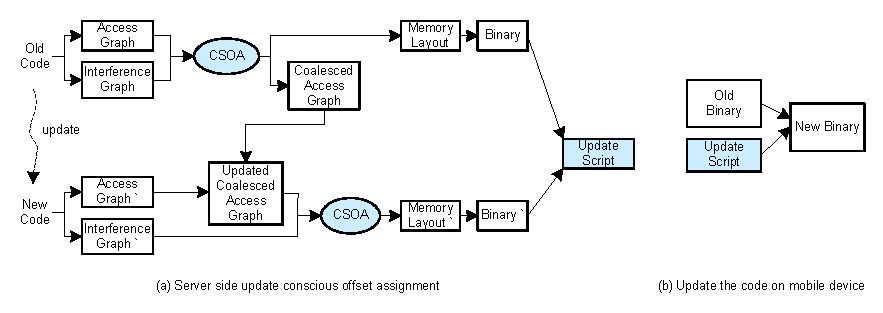
\includegraphics[scale=1.2]{./figures/icsoa-overview.eps}
\caption{An overview of Incremental Coalescing Offset Assignment (ICSOA) -based code update scheme.}
\label{ioverview}
\end{center}
\end{figure*}


The pseudo code of ICSOA is shown in Algorithm \ref{icsoaalg}. It first builds the access graphs before and after the code update, performs the CSOA algorithm, retrieves the coalesced variable assignment in $\textit{CAG}_1$, updates the new access graph $\textit{AG}_2$, resolves possible conflicts when applying the old layout to the new code, and calls CSOA again to find the new offset assignment. 

\begin{algorithm}
\caption{Incremental Coalescing-Based SOA (ICSOA)}
\singlespace
\label{icsoaalg}
\begin{algorithmic}[1]
\singlespace
\REQUIRE $\textit{AS}_1$,$\textit{AS}_2$: access sequences before and after update; \\
				 $\textit{IG}_1$,$\textit{IG}_2$: interference graphs before and after update;
\ENSURE the offset assignment.

\STATE $\textit{AG}_1$ $\leftarrow$ Build access graph using $\textit{AS}_1$;
\STATE $\textit{AG}_2$ $\leftarrow$ Build access graph using $\textit{AS}_2$;

\STATE $\textit{CAG}_1$ $\leftarrow$ CSOA($\textit{AG}_1$,$\textit{IG}_1$); 
\STATE $\textit{AG}_\textit{NEW}$ $\leftarrow$ update\_access\_graph($\textit{CAG}_1$,$\textit{AG}_2$); 
\STATE resolve\_conflicts($\textit{AG}_\textit{NEW},\textit{IG}_2$); 
\STATE $\textit{CAG}_2$ $\leftarrow$ CSOA($\textit{AG}_\textit{NEW}$, $\textit{IG}_2$);
\STATE Return offset assignment based on $\textit{CAG}_2$;
\end{algorithmic}
\end{algorithm}

\paragraph{Function  update\_access\_graph().} It combines the access graph result of the old version ($\textit{CAG}_1$) and the newly generated access graph ($\textit{AG}_2$), into a new access graph ($\textit{AG}_\textit{NEW}$).
We build $\textit{AG}_\textit{NEW}$ based on $\textit{CAG}_1$, by adding new variable nodes and removing unused nodes, so that
$\textit{AG}_\textit{NEW}$ not only represents the updated access sequence but also keeps all the coalescing offset assignment result from the old version.
Using $\textit{AG}_\textit{NEW}$ instead of $\textit{AG}_2$ as the offset assignment input helps to improve the offset assignment similarity with the previous version, and reduces the patch transmission overhead.
However, when the code change is relatively big, the energy saved by improving code similarity may be offset by the code quality loss. 
For this reason, when combining the graphs, {\it update\_access\_graph()} evaluates the number of accesses of each old variable in the new code, and extracts it from its coalesced group if the variable has more new or updated accesses than the unchanged ones. 
The intuition is to extract the variables from their old coalescing groups only if it can bring explicit benefits. 
A new node is introduced for each extracted variable. Empty group nodes will be removed from $\textit{AG}_\textit{NEW}$.
At the end, the function adjusts the weights of impacted access edges accordingly to finish the update.


\paragraph{Function resolve\_conflicts().}Due to code update, two variables that are coalesced in the old assignment may interfere with each other. We identify this as a {\em conflict} and call {\it resolve\_conflicts()} to resolve it. 

The function first orders the variables in each coalescing group, by the factor 
$$\frac{\textit{Num}_{\textit{local}\_\textit{itfs}}}{\textit{Num}_{\textit{local}\_\textit{acs}}} .$$
Here, $\textit{Num}_{\textit{local}\_\textit{itfs}}$ represents the number of interferences between the variable and the other group members, and $\textit{Num}_{\textit{local}\_\textit{acs}}$ represents the number of adjacent accesses with other group members. The function then extracts the interfering variables with a higher factor one by one until all the interferences in the group are resolved. By doing so, the variables that create more interferences but have less adjacent accesses with others are extracted first from the coalescing group. 

For each variable chosen to be extracted from the coalescing group, the function splits the live range (i.e. conflict range) into to two subranges, the original part and the newly extended part. We use the old variable name to represent the original subrange, and introduce a {\em patch variable} for the extended subrange. To ensure semantic correctness, we insert {\tt a'=a} or {\tt a=a'} to move the value between the subranges. The insertion involves memory copy and tends to incur large overhead. We will evaluate its impact in the experiments.
 
For the example in Figure~\ref{icsoa}, ICSOA combines the coalesced offset assignment (Figure \ref{icsoa}(d)) and the new access graph (Figure \ref{icsoa}(f)). Figure \ref{icsoa}(a) shows the updated access graph. As there is no conflict between the access graph and interference graph, ICSOA outputs the same coalesced assignment (Figure \ref{icsoa}(c)). In this example, the script generated from ICSOA is 71\% smaller than that of recompilation using CSOA.

\begin{figure}[htbp]
\begin{center}
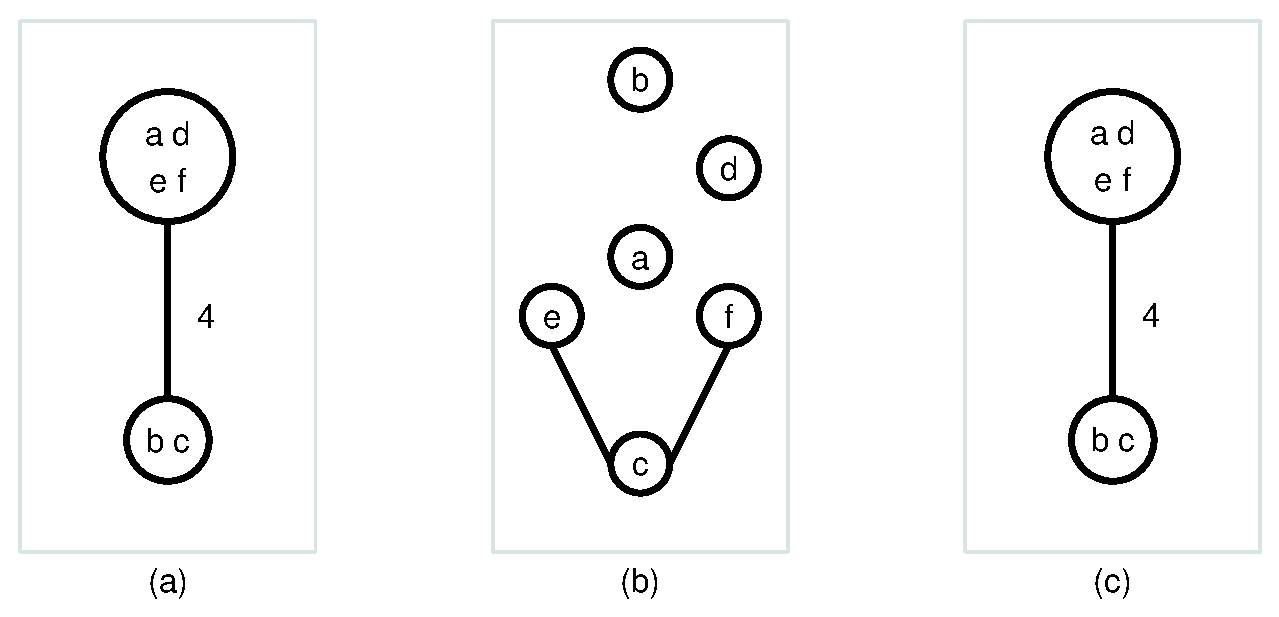
\includegraphics[scale=0.5]{./figures/icsoa.eps}
\caption{An example of ICSOA scheme:
(a) $\textit{AG}_\textit{NEW}$, the updated access graph;
(b) $\textit{IG}_2$, the new interference graph;
(c) the final offset assignment.}
\label{icsoa}
\end{center}
\vspace{-0.15in}
\end{figure}

\subsection{Register allocation problem for DSP applications}
In practice, more address registers are available on DSP chips. Keeping the address register assignment to the variables may also affect the generated code similarity.
I propose an update-conscious register allocation scheme for DSP applications here that generates a similar association between the address registers and variables
with the old version.

\subsubsection{Incremental coalescing general offset assignment (ICGOA)}
The ICSOA algorithm proposed above solves the data allocation problem for DSP applications when there is only one available address register. However, in the real DSP architecture, there are usually more than one address registers, so I propose the ICGOA algorithm here to solve more realistic problems. It is developed based on the CGOA algorithm~\cite{related:ottoni}.
The basic idea here is to assign address registers to the variables first. It divides the variables into multiple groups and the accesses to the variables in the same group will use the same address register.
Then we can use the ICSOA algorithm proposed above to allocate the variables in each partition group and generate the complete memory layout by combining the partial data allocation
results. The detailed algorithm is presented in Algorithm~\ref{icgoaalg}. 

\begin{algorithm}[htbp]
\singlespace
\begin{algorithmic}[1]
\singlespace
\REQUIRE $\textit{AS}_1$,$\textit{AS}_2$: access sequences before and after update; \\
				 $\textit{IG}_1$,$\textit{IG}_2$: interference graphs before and after update;\\
				 the number of address registers $N_{AR}$;
\ENSURE the offset assignment.\\
\COMMENT{Run CGOA over the original code}
\STATE $\textit{Partition}_1[N_{AR}] \leftarrow \textit{CGOA}(\textit{AS}_1,\textit{IG}_1,N_{AR})$;\\
\COMMENT{Remove the deleted variables and partition the newly added variables}
\STATE $\textit{Partition}_2[N_{AR}] \leftarrow  \textit{ICGOA}\_\textit{Partition}(\textit{Partition}_1[],N_{AR},\textit{AS}_2,\textit{IG}_2)$;

\COMMENT{Run ICSOA in each variable partition group}
\FOR {$i=0$ to $N_{AR}$}
\STATE $\textit{Offset}[i] \leftarrow ICSOA(\textit{Partition}_2[i],\textit{AS}_1,\textit{AS}_2,\textit{IG}_1,\textit{IG}_2)$;
\ENDFOR

\STATE Return $\textit{Offset}$;
\caption{Incremental coalescing based GOA (ICGOA).}
\label{icgoaalg}
\end{algorithmic}
\end{algorithm}

It first uses the CGOA algorithm~\cite{related:ottoni} to produce the variable partition of the old version based on the old access graph and interference graph using a heuristic based algorithm. 
The variables are sorted by the decreasing order of the {\it global interference number} $\textit{Num}_{\textit{global}\_\textit{itfs}}$, which is the total number of interferences that each variable has with the other variables. The variable that has a higher {\it global interference number} is processed earlier than the ones with lower {\it global interference numbers}, because they have more constraints.
Then, CGOA algorithm determine the partition group that the variable belongs to according to the {\it local interference numbers} $\textit{Num}_{\textit{local}\_\textit{itfs}}$. This number represents the number of interferences that this variable has with the other variables within a partition group. The {\it local interference number} between each variable and each partition group is calculated and the variable is assigned to the group that has the smallest {\it local interference number}.
This partition result is saved in $\textit{Partition}_1$ in algorithm~\ref{icgoaalg}.

\begin{figure*}[ht]
\begin{small}
\begin{eqnarray}
\textit{Num}_{\textit{global}\_\textit{itfs}}[i] = \sum_{\forall v \neq i}itf(v,i)\\
\textit{Num}_{\textit{local}\_\textit{itfs}}[i,j] = \sum_{\forall v\neq i \mbox~{and}~ v\in \textit{Partition}[j] }itf(v,i)
\end{eqnarray}
\end{small}
\caption{Objective function used in the heuristic based integration.}
\label{newObj2}
\end{figure*}

Based on the old partition result $\textit{Partition}_1$, the removed variables are first deleted from each partition. New variables are considered next. 
Same as CGOA algorithm, the new variables are first ordered by the {\it global interference number}.
Each variable tends to be assigned with the group that has the fewest {\it local interferences}.
This generated new partition $\textit{Partition}_2$ should be very similar as the old one, because it just incorporates the variable changes to the old partition.

After that, we run the ICSOA algorithm within each partition group to generate the memory layout for the variables inside each group.
The ICSOA results are then combined to form the final result.


